%% LaTeX2e class for student theses
%% sections/content.tex
%%
%% Karlsruhe University of Applied Sciences
%% Faculty of  Computer Science and Business Information Systems
%% Distributed Systems (vsys)
%%
%% Prof. Dr. Christian Zirpins
%% christian.zirpins@hs-karlsruhe.de
%%
%%
%% Version 0.2, 2017-11-15
%%
%% --------------------------------------------------------
%% | Derived from sdqthesis by Erik Burger burger@kit.edu |
%% --------------------------------------------------------

\chapter{Grundlagen zur sicheren Umsetzung dezentraler sozialer Netzwerke}
\label{ch:fundamentals}
\iflanguage{english}{
	
}{
	\glqq \gls{AS2}\grqq~beinhaltet Modelle für Aktoren, Aktivitäten, Intransitiven Aktivitäten, Objekte, Links, Sammlungen, Natürliche Sprachwerte (Strings) und für Internationalisierung. Das Kernvokabular von \gls{AS2} wird durch \gls{asv} erweitert. Dazu gehören verschiedene Aktivitätstypen wie z.B. \glqq Accept\grqq,\glqq Add\grqq,\glqq Remove\grqq,\glqq Delete\grqq~und \glqq Create\grqq\footnote{\href{https://www.w3.org/TR/activitystreams-vocabulary/}{activity-types https://www.w3.org/TR/activitystreams-vocabulary/}}, um Aktorentypen wie \glqq Person\grqq, \glqq Application\grqq~und \glqq Group\grqq\footnote{\href{https://www.w3.org/TR/activitystreams-vocabulary/}{actor-types https://www.w3.org/TR/activitystreams-vocabulary/}} sowie um verschiedenste Objekttypen wie \glqq Article\grqq, \glqq Event\grqq, \glqq Note\grqq~und \glqq Relationship\grqq\footnote{\href{https://www.w3.org/TR/activitystreams-vocabulary/}{object-types https://www.w3.org/TR/activitystreams-vocabulary/}}.\\
	\todo{Sammlungen beschreiben!}
	
	\todo{Wusste eben nicht wie ich das anders machen soll außer als Fußnote. Wie könnte ich ein "siehe Weblink" gestalten??? Weil alles hier nochmal aufzulisten wäre denke ich nicht gut..}
	%% Use Case Diagram
	\todo{Meinst du mit Übersichtsdiagramm, UseCase Diagramme mit z.B. Client to Server Interaktionen als Package und senden von Aktivitäten an die Outbox sowie empfangen von der Inbox als Usecases??? usw..}
}
\section{ActivityPub Standard}
	\iflanguage{english}{
		
	}{
		ActivityPub definiert zwei Protokollschichten, sowie Konzepte, Sammlungen und Interaktionen für dezentrale soziale Netzwerke. Eine Protokollschicht ist das Client-zu-Server Protokoll (Social API), um Clients den Zugriff auf einen Server zu ermöglichen sowie zum entgegennehmen von Anfragen. Die zweite Protokollschicht besteht aus dem förderierten Server-zu-Server Protkoll (Federation Protocol), welches den einzelnen Instanzen von dezentralen sozialen Netzwerken den Austausch von Inhalten untereinander gestattet. ActivityPub setzt auf bereits bestehende Empfehlungen des \gls{w3c} auf, welche teilweise auch von der \gls{swwg} entwickelt wurden wie zB. \gls{asc} und \gls{asv}.\\
		
		Auch andere Technologien wie \gls{JSON-LD} werden benutzt um die Erweiterbarkeit zu gewährleisten. Über neue Ontologien (Vokabulare) können weitere syntaktische Definitionen und semantische Beschreibungen zu den bestehenden hinzugefügt werden. Diese Vokabulare können im Kontext des \gls{JSON-LD} Objektes, angegeben werden.\\
		
		\todo{Stimmt das mit den Ontologien???}
		\todo{Beispiel Context Abbildung mit erweitertem Context???}
	}
	\subsection{Bestandteile des Protokolls}
		Das Client-zu-Server sowie förderierte Server-zu-Server Protokoll können unabhängig voneinander implementiert werden. Ersteres besteht aus einem Client und Server Teil.\\
		
		In ActivityPub werden Benutzer als \glqq Aktoren\grqq(actors) dargestellt. Diese können nicht nur Personen, sondern auch Applikationen, Organisationen, Gruppen und Services sein\cite{activityStreamsCoreActors}. Jedes Aktoren Objekt muss eine \glqq Inbox\grqq~und \glqq Outbox\grqq, welche geordnete Sammlungen sein müssen, sowie eine ID und ein Typ besitzen\cite{activityPubActor}. Die ID muss global einzigartig sein. Dies kann garantiert werden durch eine Domänen und Protokoll bezogene URI oder IRI wie zum Beispiel \glqq https://example.org/users/alice\grqq oder \glqq https://example.org/alice/posts/2\grqq. %http://fusion.cs.uni-jena.de/fusion/blog/2016/11/18/iri-uri-url-urn-and-their-differences/
		Die Typ Eigenschaft kann variieren zwischen den fünf oben genannten.
	
		\lstinputlisting[caption={Beispiel Aktoren Objekt}, label=listing::actor, language=JavaScript]{resources/mastodon-macu.json}
	
	\subsection{Zugehörige Standards und Komponenten}
		ActivityPub benutzt die ActivityStreams Daten Syntax und das Vokabular. Zusätzlich kann ein Sicherheitsvokabular benutzt werden. Am 22 April 2016 hat die \glqq W3C Community Group\grqq~ einen Entwurfsbericht herausgebracht. Durch diesen wird neue Syntax und Semantik definiert um Internet basierten Applikationen das Verschlüsseln, Entschlüsseln sowie digitale signieren und verifizieren von verlinkten Daten (Linked Data) zu ermöglichen. "Es enthält auch Vokabeln für die Erstellung und Verwaltung einer dezentralen Public-Key-Infrastruktur über das Internet." \cite{security-vocab-linked-data}. Ein Anwendungsfall ist das holen des öffentlichen Schlüssels eines Nutzers, über dessen Aktoren Objekt, um eine von Nutzer gesendete Nachricht zu verifizieren.
		
		\gls{JSON-LD} ist eine Erweiterung des JSON Formates um verlinkte Daten zu Repräsentieren. JSON an sich, ist ein Format welches im Web häufig Anwendung findet um Daten auszutauschen. Im Kern sind \gls{AS2} auch \gls{JSON-LD} Objekte. Der \gls{AS2} Kontext definiert verschiedene Klassen und Eigenschaften, von denen nicht alle benutzt werden. Typische Klassen sind \glqq Activity\grqq, \glqq Link\grqq~und \glqq OrderedCollection\grqq. Ein Beispiel \gls{AS2} Objekt sieht wie folgt aus: 	
		\lstinputlisting[caption={Beispiel \gls{AS2} Objekt}, label=listing::as2-object, language=JavaScript]{resources/example-as2-object.json}
		
		Über ein Profil ist es möglich, einem \glqq Media-Type\grqq~zusätzliche Semantik hinzuzufügen https://tools.ietf.org/html/rfc6906.\\
		
		Es ist auch möglich ein Profil anstatt eines Aktoren Objektes anzugeben.
		%https://www.w3.org/TR/activitystreams-vocabulary/#dfn-profile 
		
		\todo{Die letzten beiden Absätze gehören zur Frage..\\Mir ist nicht ganz klar was mit dem Profil gemeint ist.. laut dem RFC am Ende des dritten Absatzes, wird das verwendet um neue Semantik hinzuzufügen.. Blos wird dafür doch schon der JSON-LD Context benutzt "@context": "https://www.w3.org/ns/activitystreams"?}
\section{Client-zu-Server Kommunikation}
	Der Client interagiert über zwei Schnittstellen mit dem Server. Er kann sich per HTTP GET Anfrage auf seine eigene \glqq Inbox\grqq~die neusten an ihn adressierten Inhalte holen und über eine HTTP POST Anfrage auf seine \glqq Outbox\grqq~neue Inhalte erstellen.
	\begin{figure}[h]
		\centering
		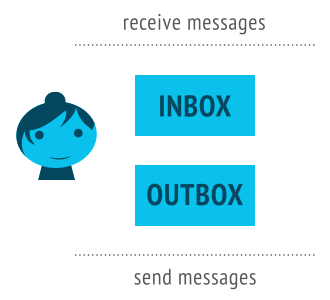
\includegraphics[scale=0.6]{figures/inbox-outbox.png}
		\label{Client zu Server Interaktionen}
		\caption{Interaktionen des Client mit dem Server}
	\end{figure}\\
	Um neue Aktivitäten an seine Folgenden, direkt an einzelne Personen, sichtbar innerhalb der Domain oder unangemeldet für alle zugänglich zu veröffentlichen, kann der Client eine HTTP POST Anfrage an seine \glqq Outbox\grqq~senden mit einer Aktivität oder einem \gls{AS2} Objekt als Inhalt. Der Client muss mehrere Aufgaben, wie in \ref{client-to-server:client-part} beschrieben, übernehmen.
	
	\subsection{Client Teil}
	\label{client-to-server:client-part}
		%%The client, represented as an actor, interacts with the server in two ways. First through sending a HTTP GET request with an Activity object to an actors inbox and through HTTP POST an Activity object to an actors outbox. An inbox and outbox must be a OrderedCollection.
		\begin{itemize}
			\item Auffinden der URL über das Aktoren Objekt
			\item Serialisieren der Daten in eine Aktivität oder \gls{AS2} Objekt
			\item Adressieren von Aktivitäten oder \gls{AS2} Objekten
			\item Eine HTTP POST Anfrage mit \glqq Content-Type: application/ld+json: profile="https://w3.org/ns/activitystreams"\grqq~oder \glqq Content-Type: application/activity+json: profile="https://w3.org/ns/activitystreams"\grqq~an seine \glqq Outbox\grqq~absetzen können
			\item Bei den Aktivitätstypen CREATE, UPDATE, DELETE, FOLLOW, ADD, REMOVE, LIKE, BLOCK, UNDO wird die \glqq object\grqq~Eigenschaft bereitgestellt
			\item Die \glqq target\grqq~Eigenschaft wird bei den Aktivitätstypen ADD und REMOVE bereitgestellt
			\item Anfragen müssen mit den Zugangsdaten des Nutzer, zu dem die \glqq Outbox\grqq~gehört, authentifiziert werden
		\end{itemize}
		Die beiden Eigenschaften \glqq target\grqq~und \glqq object\grqq~müssen bei verschiedensten Aktivitätstypen bereitgestellt werden. Zum Beispiel muss die \glqq target\grqq~Eigenschaft bei den Aktivitätstypen ADD und REMOVE angegeben werden.\\
		
		Der Client Teil des Client-zu-Server Protokolls beinhaltet die oben gelisteten Aufgaben. Zusammengefasst muss sich der Client um das Entdecken von Endpunkten - Inbox/Outbox - über Aktorenobjekte, das Addressieren von Aktivitäten und Serialisieren von Daten zu Aktivitäten oder \gls{AS2} Objekten sowie um das setzen der entsprechenden Kopfzeilen (Mittlerer Teil der obigen Auflistung) und Absenden der HTTP POST Anfrage kümmern. Außerdem muss bei HTTP GET Anfragen an den Server die \glqq ACCEPT: application/ld+json\grqq~Kopfzeile gesetzt sein.\\
		
		Wenn ein Nutzer z.B. ein \glqq Post\grqq~erstellt, wird der \glqq Post\grqq entweder zu einem \gls{AS2} Objekt oder direkt zu einer Aktivität serialisiert. Anschließend wird das serialisierte Objekt adressiert. Dies geschieht über das beschaffen der \glqq Inboxen\grqq~über die Aktoren Objekte der Empfänger. Sobald die Endpunkte bekannt sind, können diese in das \glqq to\grqq Feld in dem Objekt geschrieben werden. Zum Schluß wird eine authentifizierte HTTP POST Anfrage, wie in Element 4 der obigen Liste beschrieben, abgesetzt.

	\subsection{Server Teil} 
		Zu den Aufgaben des Serverteils gehören das Annehmen von HTTP POST Anfragen auf die \glqq Outbox\grqq~eines Nutzers und das verifizieren ob der Nutzer berechtigt ist diese Anfrage zu tätigen. Weiter werden die \glqq Inbox\grqq~Endpunkte bereitgestellt um authentifizierten Nutzern den Zugriff auf die neusten Inhalte zu geben. Der Server Teil des Client-zu-Server Protokolls bezieht sich nur auf eine Domäne. Für das verteilen von Aktivitäten an andere Server muss zusätzlich das förderierte Server-zu-Server Protokoll implementiert werden.

\section{Server-zu-Server Kommunikation}
	\begin{figure}[h]
		\centering
		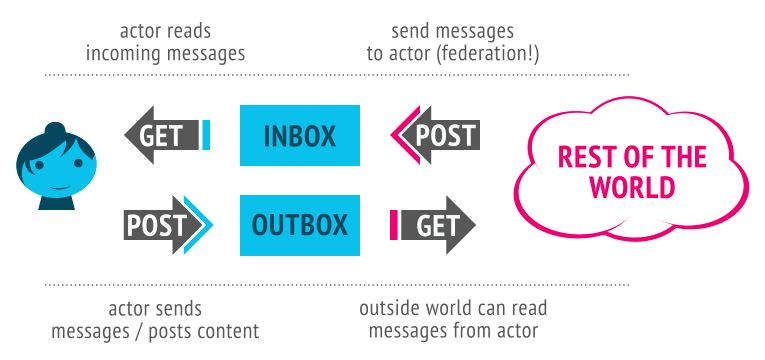
\includegraphics[scale=0.55]{figures/client-server-federated.png}
		\label{Client zu Server und Server zu Server Interaktionen}
		\caption{Schnittstellen des ActivityPub Protokolls}
	\end{figure}
	Bei der Server-zu-Server Kommunikation bestehen die Hauptaufgaben im annehmen und zustellen von HTTP POST Anfragen auf die \glqq Inboxen\grqq~und \glqq Outboxen\grqq~der Nutzer und im Weiterleiten von Aktivitäten die der Server nicht zustellen kann. Empfängt dieser eine Aktivität welche nicht an die zugehörige Domäne gerichtet ist, wird die Aktivität an den zur Domäne gehörigen Server gesendet. Dazu kommt das Bereitstellen der \glqq Outbox\grqq~Sammlungen.
	
\section{Authentifizierung und Datenintegrität}
	Für die Authentifizierung und zum sichern der Datenintegrität definiert der Standard keine Mechanismen. Es gibt allerdings \glqq Best Practices\grqq~für die Umsetzung dieser Anforderungen.\\
	
	Zum einen werden bei der Client-zu-Server Authentifizierung \glqq OAuth 2.0\grqq~Tokens benutzt, zum anderen auf der Server Seite \glqq HTTP\grqq~oder \glqq Linked Data Signatures\grqq zur Sicherstellung der Datenintegrität.\\
	
	\todo{Datenintegrität}
	
	\todo{OAuth 2.0}
	
	\todo{HTTP Signaturen}
	Um sicherzustellen das HTTP Anfragen beim Transport nicht verändert wurden, können HTTP Signaturen verwendet werden.\\
	\todo{Linked Data Signaturen}
	Wenn ein Objekt nicht nur vom Client zum Server gesendet, sondern auch zwischen Servern untereinander weitergeleitet werden soll wird zum Sicherstellen der Datenintegrität ein anderes Verfahren benötig als HTTP Signaturen. Die \glqq Best Practices\grqq~empfehlen für solche Fälle \glqq Linked Data Signatures\grqq. Der größte Unterschied zwischen HTTP Signaturen und \glqq Linked Data Signatures\grqq~besteht darin, welche Daten zum Erstellen der Signatur verwendet werden. Bei HTTP Signaturen sind es die Kopfzeilen. Mit \glqq Linked Data Signatures\grqq~kann auch das Objekt selbst, also der Payload einer HTTP Anfrage, anstatt nur die Kopfzeilen, zum signieren verwendet werden.
